\documentclass[a4paper,10pt]{article}

\usepackage[ansinew]{inputenc}
\usepackage[spanish]{babel}
\usepackage{graphicx}
\usepackage{listings}
\usepackage{appendix}
\usepackage{pdfpages}
\usepackage{fancyhdr}
\pagestyle{fancy}

\begin{document}

\lhead{\fancyplain{}{Base de Datos 75.15}}
\rhead{\fancyplain{}{Trabajo Pr\'actico Grupal}}

\setcounter{page}{2}

\newpage
\thispagestyle{empty}
\tableofcontents

\newpage
\section{Modelo Entidad Relaci\'on}
  \subsection{Diagrama}
  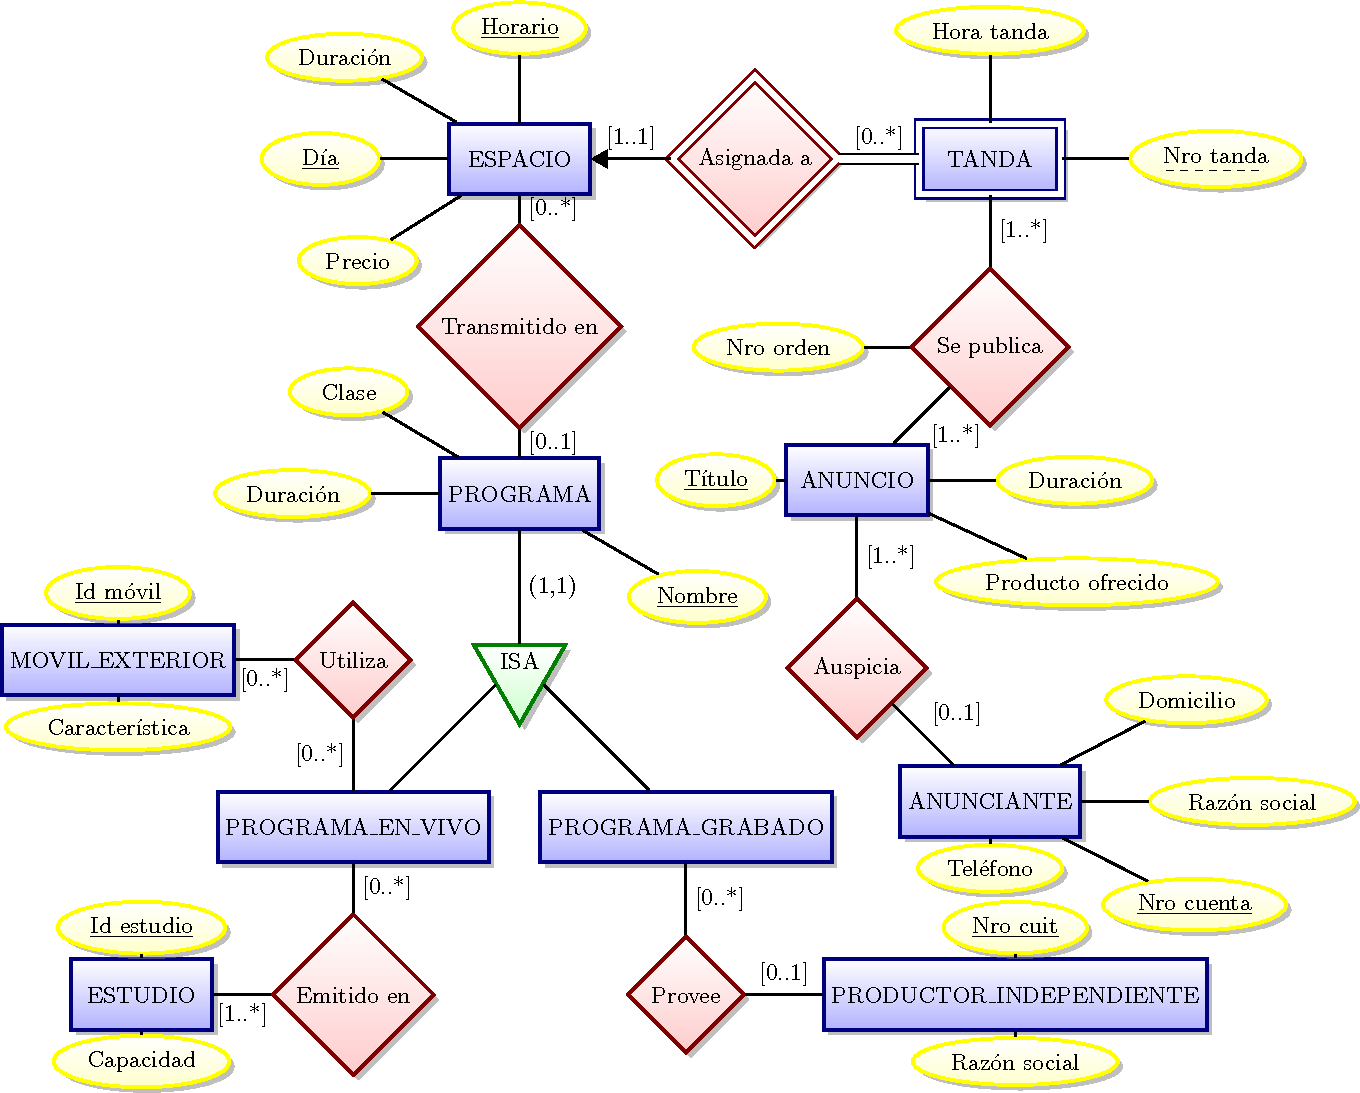
\includegraphics[width=10cm]{ModeloE-R/ModeloE-R.png}
  
  \subsection{Hip\'otesis}
    \begin{enumerate}
      \item Cada m\'ovil de exterior posee un id que lo identifica un\'ivocamente. 
      \item Un programa puede ser en vivo o grabado.
      \item S\'olo los programas en vivo poseen estudios de emisi\'on.
    \end{enumerate}
    
  \subsection{Diccionario}
    \subsubsection{Entidades}
    \begin{flushleft}
      \begin{large} \bf{Espacio} \end{large}
    \end{flushleft}
      \begin{tabular}{| p{2cm} | p{9cm} |}
	\hline
	\multicolumn{2}{|l|}{\bf{Descripci\'on:}} \\
	\hline
	\multicolumn{2}{|l|}{Un espacio es una divisi\'on del horario de transmisi\'on del canal.} \\
	\hline	
	\multicolumn{2}{|l|}{\bf{Especificaci\'on de atributos:}} \\
	\hline
	- D\'ia & El d\'ia en el que se emite el espacio. \\
	\hline \hline
	- Horario & El horario en el que se emite el espacio. \\
	\hline \hline
	- Duraci\'on & La duraci\'on del espacio.\\
	\hline \hline
	- Precio & El precio por segundo en el aire del espacio.\\
	\hline
	\multicolumn{2}{|l|}{\bf{Especificaci\'on de identificador \'unico:}} \\
	\hline
	\multicolumn{2}{|l|}{- D\'ia + Horario} \\
	\hline
      \end{tabular}
    
    \begin{flushleft}
      \begin{large} \bf{Tanda} \end{large}
    \end{flushleft}
      \begin{tabular}{| p{2cm} | p{9cm} |}
	\hline
	\multicolumn{2}{|l|}{\bf{Descripci\'on:}} \\
	\hline
	\multicolumn{2}{|l|}{Un tanda es un espacio donde se publicitan anuncios.} \\
	\hline	
	\multicolumn{2}{|l|}{\bf{Especificaci\'on de atributos:}} \\
	\hline
	- Hora tanda & La hora de comienzo de la tanda. \\
	\hline \hline
	- Nro tanda & El n\'umero de tanda correspondiente a un programa. \\
	\hline
	\multicolumn{2}{|l|}{\bf{Especificaci\'on de identificador \'unico:}} \\
	\hline
	\multicolumn{2}{|l|}{- D\'ia + Hora tanda + Nro tanda} \\
	\hline
      \end{tabular}

    \begin{flushleft}
      \begin{large} \bf{Anuncio} \end{large}
    \end{flushleft}
      \begin{tabular}{| p{2cm} | p{9cm} |}
	\hline
	\multicolumn{2}{|l|}{\bf{Descripci\'on:}} \\
	\hline
	\multicolumn{2}{|l|}{Un anuncio es un espacio, dentro de una tanda, destinado a dar a conocer} \\
	\multicolumn{2}{|l|}{un producto.} \\
	\hline	
	\hline	
	\multicolumn{2}{|l|}{\bf{Especificaci\'on de atributos:}} \\
	\hline
	- T\'itulo & El t\'itulo del anuncio. \\
	\hline \hline
	- Duraci\'on & La duraci\'on del anuncio. \\
	\hline \hline
	- Producto \newline ofrecido & El producto ofrendido del anuncio. \\
	\hline
	\multicolumn{2}{|l|}{\bf{Especificaci\'on de identificador \'unico:}} \\
	\hline
	\multicolumn{2}{|l|}{- T\'itulo} \\
	\hline
      \end{tabular}

    \begin{flushleft}
      \begin{large} \bf{Anunciante} \end{large}
    \end{flushleft}
      \begin{tabular}{| p{2cm} | p{9cm} |}
	\hline
	\multicolumn{2}{|l|}{\bf{Descripci\'on:}} \\
	\hline
	\multicolumn{2}{|l|}{Un anunciante auspicia a lo sumo un producto, mediante un anuncio.} \\
	\hline	
	\multicolumn{2}{|l|}{\bf{Especificaci\'on de atributos:}} \\
	\hline
	- Nro cuenta & El n\'umero de cuenta del anunciante. \\
	\hline \hline
	- Domicilio & El domicilio del anunciante. \\
	\hline \hline
	- Raz\'on \newline social & La raz\'on social del anunciante. \\
	\hline \hline
	- Tel\'efono & El tel\'efono del anunciate. \\
	\hline
	\multicolumn{2}{|l|}{\bf{Especificaci\'on de identificador \'unico:}} \\
	\hline
	\multicolumn{2}{|l|}{- Nro cuenta} \\
	\hline
      \end{tabular}

    \begin{flushleft}
      \begin{large} \bf{Asi con todos........} \end{large}
    \end{flushleft}
   
    \subsubsection{Interrelaciones}


\newpage
\section{Transformaci\'on del Modelo E-R a un Modelo Relacional}

%APENDICES
\appendix
\newpage
\section{Enunciado}
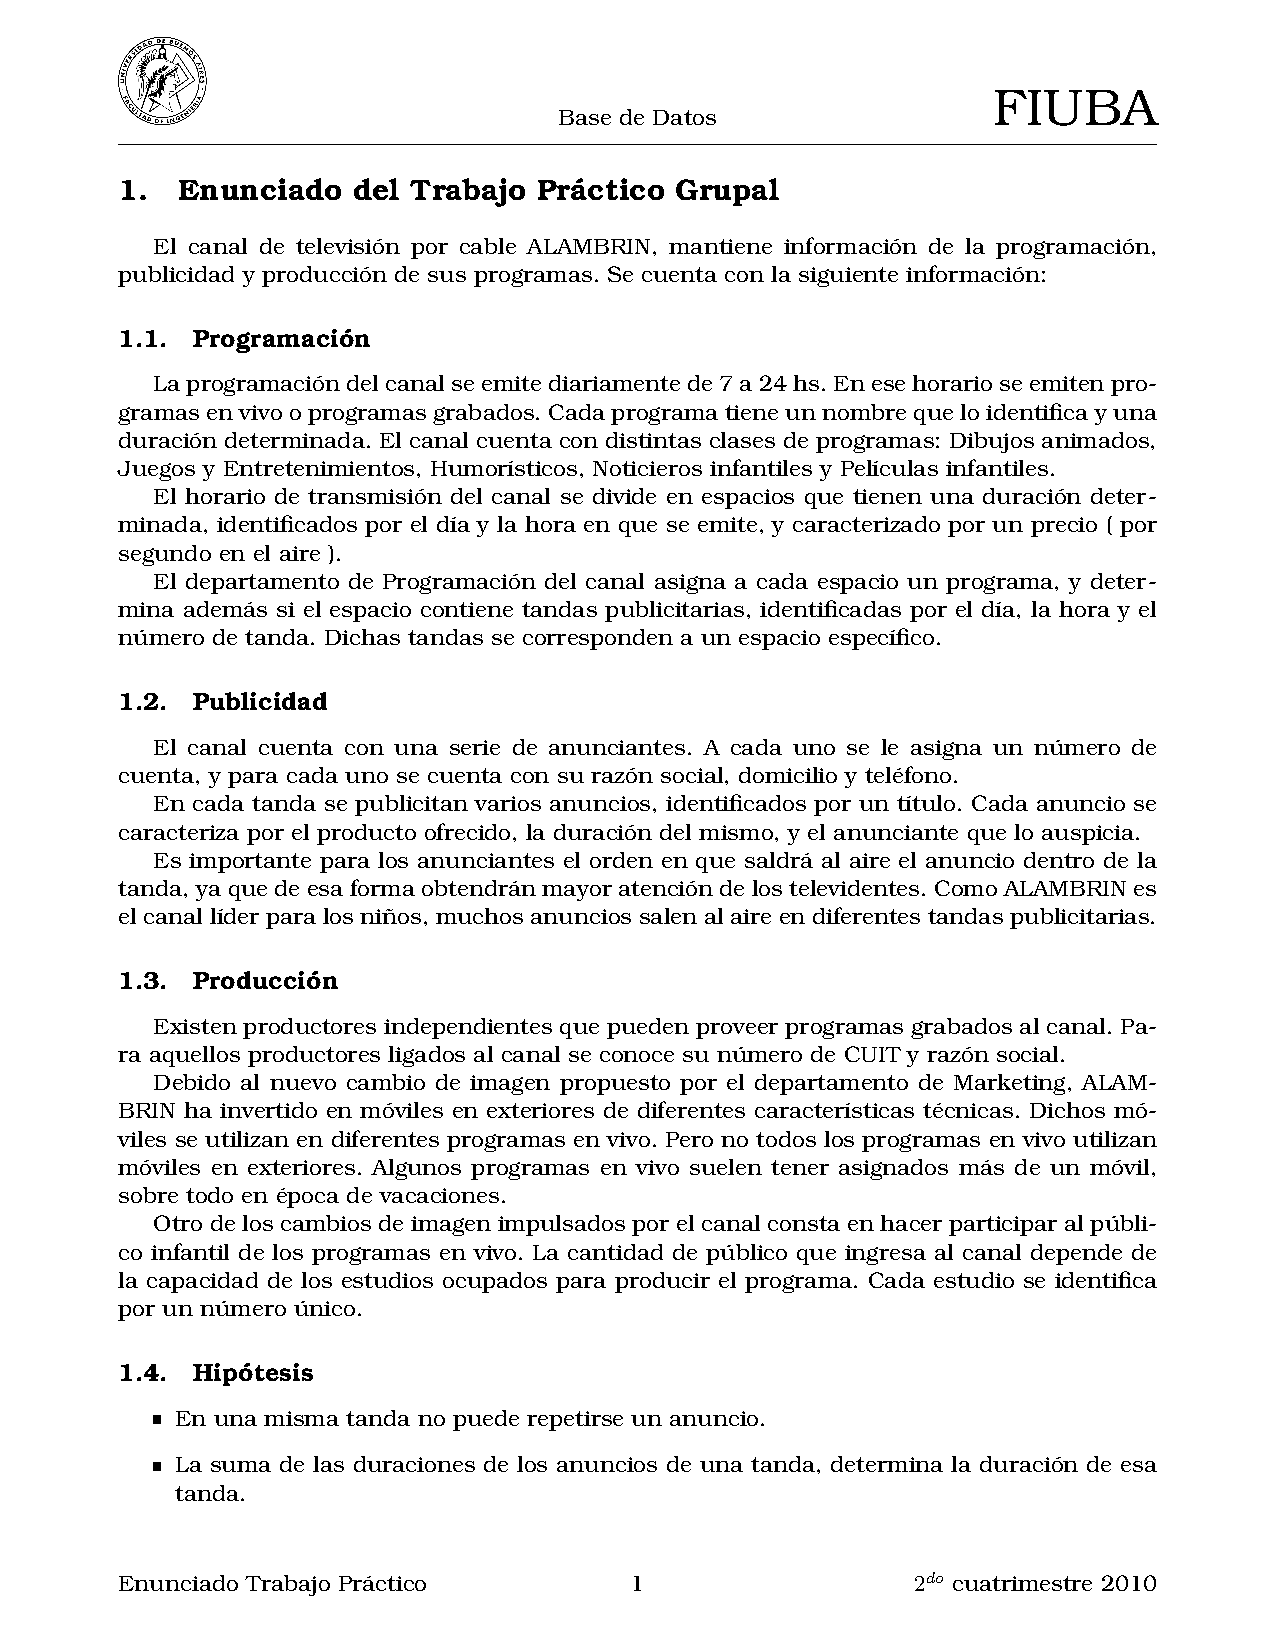
\includepdf[pages=1-2, scale=0.8, pagecommand={\thispagestyle{plain}}]{EnunciadoBD.pdf}

\end{document}
